
\documentclass[letterpaper,hide notes,xcolor={table,svgnames},pdftex]{beamer}
\def\showexamples{t}


%\usepackage[svgnames]{xcolor}

%% Demo talk
%\documentclass[letterpaper,notes=show]{beamer}

\usecolortheme{crane}
\setbeamertemplate{navigation symbols}{}

\usetheme{MyPittsburgh}
%\usetheme{Frankfurt}

%\usepackage{tipa}

\usepackage{hyperref}
\usepackage{graphicx,xspace}
\usepackage[normalem]{ulem}

\newcommand\SF[1]{$\bigstar$\footnote{SF: #1}}



\newcounter{tmpnumSlide}
\newcounter{tmpnumNote}

% old question code
%\newcommand\question[1]{{$\bigstar$ \small \onlySlide{2}{#1}}}
% \newcommand\nquestion[1]{\ifdefined \presentationonly \textcircled{?} \fi \note{\par{\Large \textbf{?}} #1}}
% \newcommand\nanswer[1]{\note{\par{\Large \textbf{A}} #1}}


 \newcommand\mnote[1]{%
   \addtocounter{tmpnumSlide}{1}
   \ifdefined\showcues {~\tiny\fbox{\arabic{tmpnumSlide}}}\fi
   \note{\setlength{\parskip}{1ex}\addtocounter{tmpnumNote}{1}\textbf{\Large \arabic{tmpnumNote}:} {#1\par}}}

\newcommand\mmnote[1]{\note{\setlength{\parskip}{1ex}#1\par}}

%\newcommand\mnote[2][]{\ifdefined\handoutwithnotes {~\tiny\fbox{#1}}\fi
% \note{\setlength{\parskip}{1ex}\textbf{\Large #1:} #2\par}}

%\newcommand\mnote[2][]{{\tiny\fbox{#1}} \note{\setlength{\parskip}{1ex}\textbf{\Large #1:} #2\par}}

\newcommand\mquestion[2]{{~\color{red}\fbox{?}}\note{\setlength{\parskip}{1ex}\par{\Large \textbf{?}} #1} \note{\setlength{\parskip}{1ex}\par{\Large \textbf{A}} #2\par}\ifdefined \presentationonly \pause \fi}

\newcommand\blackboard[1]{%
\ifdefined   \showblackboard
  {#1}
  \else {\begin{center} \fbox{\colorbox{blue!30}{%
         \begin{minipage}{.95\linewidth}%
           \hspace{\stretch{1}} Some space intentionally left blank; done at the blackboard.%
         \end{minipage}}}\end{center}}%
         \fi%
}



%\newcommand\q{\tikz \node[thick,color=black,shape=circle]{?};}
%\newcommand\q{\ifdefined \presentationonly \textcircled{?} \fi}

\usepackage{listings}
\lstset{%
  keywordstyle=\bfseries,
  aboveskip=15pt,
  belowskip=15pt,
  captionpos=b,
  identifierstyle=\ttfamily,
  escapeinside={(*@}{@*)},
  stringstyle=\ttfamiliy,
  frame=lines,
  numbers=left, basicstyle=\scriptsize, numberstyle=\tiny, stepnumber=0, numbersep=2pt}

\usepackage{siunitx}
\newcommand\sius[1]{\num[group-separator = {,}]{#1}\si{\micro\second}}
\newcommand\sims[1]{\num[group-separator = {,}]{#1}\si{\milli\second}}
\newcommand\sins[1]{\num[group-separator = {,}]{#1}\si{\nano\second}}
\sisetup{group-separator = {,}, group-digits = true}

%% -------------------- tikz --------------------
\usepackage{tikz}
\usetikzlibrary{positioning}
\usetikzlibrary{arrows,backgrounds,automata,decorations.shapes,decorations.pathmorphing,decorations.markings,decorations.text}

\tikzstyle{place}=[circle,draw=blue!50,fill=blue!20,thick, inner sep=0pt,minimum size=6mm]
\tikzstyle{transition}=[rectangle,draw=black!50,fill=black!20,thick, inner sep=0pt,minimum size=4mm]

\tikzstyle{block}=[rectangle,draw=black, thick, inner sep=5pt]
\tikzstyle{bullet}=[circle,draw=black, fill=black, thin, inner sep=2pt]

\tikzstyle{pre}=[<-,shorten <=1pt,>=stealth',semithick]
\tikzstyle{post}=[->,shorten >=1pt,>=stealth',semithick]
\tikzstyle{bi}=[<->,shorten >=1pt,shorten <=1pt, >=stealth',semithick]

\tikzstyle{mut}=[-,>=stealth',semithick]

\tikzstyle{treereset}=[dashed,->, shorten >=1pt,>=stealth',thin]

\usepackage{ifmtarg}
\usepackage{xifthen}
\makeatletter
% new counter to now which frame it is within the sequence
\newcounter{multiframecounter}
% initialize buffer for previously used frame title
\gdef\lastframetitle{\textit{undefined}}
% new environment for a multi-frame
\newenvironment{multiframe}[1][]{%
\ifthenelse{\isempty{#1}}{%
% if no frame title was set via optional parameter,
% only increase sequence counter by 1
\addtocounter{multiframecounter}{1}%
}{%
% new frame title has been provided, thus
% reset sequence counter to 1 and buffer frame title for later use
\setcounter{multiframecounter}{1}%
\gdef\lastframetitle{#1}%
}%
% start conventional frame environment and
% automatically set frame title followed by sequence counter
\begin{frame}%
\frametitle{\lastframetitle~{\normalfont(\arabic{multiframecounter})}}%
}{%
\end{frame}%
}
\makeatother

\makeatletter
\newdimen\tu@tmpa%
\newdimen\ydiffl%
\newdimen\xdiffl%
\newcommand\ydiff[2]{%
    \coordinate (tmpnamea) at (#1);%
    \coordinate (tmpnameb) at (#2);%
    \pgfextracty{\tu@tmpa}{\pgfpointanchor{tmpnamea}{center}}%
    \pgfextracty{\ydiffl}{\pgfpointanchor{tmpnameb}{center}}%
    \advance\ydiffl by -\tu@tmpa%
}
\newcommand\xdiff[2]{%
    \coordinate (tmpnamea) at (#1);%
    \coordinate (tmpnameb) at (#2);%
    \pgfextractx{\tu@tmpa}{\pgfpointanchor{tmpnamea}{center}}%
    \pgfextractx{\xdiffl}{\pgfpointanchor{tmpnameb}{center}}%
    \advance\xdiffl by -\tu@tmpa%
}
\makeatother
\newcommand{\copyrightbox}[3][r]{%
\begin{tikzpicture}%
\node[inner sep=0pt,minimum size=2em](ciimage){#2};
\usefont{OT1}{phv}{n}{n}\fontsize{4}{4}\selectfont
\ydiff{ciimage.south}{ciimage.north}
\xdiff{ciimage.west}{ciimage.east}
\ifthenelse{\equal{#1}{r}}{%
\node[inner sep=0pt,right=1ex of ciimage.south east,anchor=north west,rotate=90]%
{\raggedleft\color{black!50}\parbox{\the\ydiffl}{\raggedright{}#3}};%
}{%
\ifthenelse{\equal{#1}{l}}{%
\node[inner sep=0pt,right=1ex of ciimage.south west,anchor=south west,rotate=90]%
{\raggedleft\color{black!50}\parbox{\the\ydiffl}{\raggedright{}#3}};%
}{%
\node[inner sep=0pt,below=1ex of ciimage.south west,anchor=north west]%
{\raggedleft\color{black!50}\parbox{\the\xdiffl}{\raggedright{}#3}};%
}
}
\end{tikzpicture}
}


%% --------------------

%\usepackage[excludeor]{everyhook}
%\PushPreHook{par}{\setbox0=\lastbox\llap{MUH}}\box0}

%\vspace*{\stretch{1}

%\setbox0=\lastbox \llap{\textbullet\enskip}\box0}

\setlength{\parskip}{\fill}

\newcommand\noskips{\setlength{\parskip}{1ex}}
\newcommand\doskips{\setlength{\parskip}{\fill}}

\newcommand\xx{\par\vspace*{\stretch{1}}\par}
\newcommand\xxs{\par\vspace*{2ex}\par}
\newcommand\tuple[1]{\langle #1 \rangle}
\newcommand\code[1]{{\sf \footnotesize #1}}
\newcommand\ex[1]{\uline{Example:} \ifdefined \presentationonly \pause \fi
  \ifdefined\showexamples#1\xspace\else{\uline{\hspace*{2cm}}}\fi}

\newcommand\ceil[1]{\lceil #1 \rceil}


\AtBeginSection[]
{
   \begin{frame}
       \frametitle{Outline}
       \tableofcontents[currentsection]
   \end{frame}
}



\pgfdeclarelayer{edgelayer}
\pgfdeclarelayer{nodelayer}
\pgfsetlayers{edgelayer,nodelayer,main}

\tikzstyle{none}=[inner sep=0pt]
\tikzstyle{rn}=[circle,fill=Red,draw=Black,line width=0.8 pt]
\tikzstyle{gn}=[circle,fill=Lime,draw=Black,line width=0.8 pt]
\tikzstyle{yn}=[circle,fill=Yellow,draw=Black,line width=0.8 pt]
\tikzstyle{empty}=[circle,fill=White,draw=Black]
\tikzstyle{bw} = [rectangle, draw, fill=blue!20, 
    text width=4em, text centered, rounded corners, minimum height=2em]
    
    \newcommand{\CcNote}[1]{% longname
	This work is licensed under the \textit{Creative Commons #1 3.0 License}.%
}
\newcommand{\CcImageBy}[1]{%
	\includegraphics[scale=#1]{creative_commons/cc_by_30.pdf}%
}
\newcommand{\CcImageSa}[1]{%
	\includegraphics[scale=#1]{creative_commons/cc_sa_30.pdf}%
}
\newcommand{\CcImageNc}[1]{%
	\includegraphics[scale=#1]{creative_commons/cc_nc_30.pdf}%
}
\newcommand{\CcGroupBySa}[2]{% zoom, gap
	\CcImageBy{#1}\hspace*{#2}\CcImageNc{#1}\hspace*{#2}\CcImageSa{#1}%
}
\newcommand{\CcLongnameByNcSa}{Attribution-NonCommercial-ShareAlike}

\newenvironment{changemargin}[1]{% 
  \begin{list}{}{% 
    \setlength{\topsep}{0pt}% 
    \setlength{\leftmargin}{#1}% 
    \setlength{\rightmargin}{1em}
    \setlength{\listparindent}{\parindent}% 
    \setlength{\itemindent}{\parindent}% 
    \setlength{\parsep}{\parskip}% 
  }% 
  \item[]}{\end{list}} 



\usepackage{alltt}

\title{Lecture 11 --- Multithreading}

\author{Jeff Zarnett\\ \small \texttt{jzarnett@uwaterloo.ca}}
\institute{Department of Electrical and Computer Engineering \\[-1ex]
  University of Waterloo}
\date{\today}


\begin{document}


\begin{frame}
  \titlepage

\end{frame}

\begin{frame}
\frametitle{Objective}

\begin{changemargin}{1cm}
Goal: a brief introduction to multithreading
\mnote{Multithreading is a huge topic and we are not going to be able to cover it in great detail in one lecture. This will come up in much more detail later on in your education, and maybe in your work terms.}
\end{changemargin}
\end{frame}

\begin{frame}
\frametitle{About Multithreading}
\begin{changemargin}{1cm}
First definition: a \alert{Process}.

Process has three main components:\\
\quad An executable program,\\
\quad Data created/needed by the program, and\\
\quad Execution context of the program \mnote{files opened, resources allocated, etc}

A process has at least one \alert{Thread}.

\end{changemargin}
\end{frame}

\begin{frame}
\frametitle{About Multithreading}
\begin{changemargin}{1cm}
Thread: A short form of \alert{Thread of Execution}.

A sequence of executable commands that can be scheduled to run on the CPU. \mnote{In ECE 150 and most of the other classes you will take at Waterloo, the code you write will have only one thread; that is, your program's code is executed one statement at a time.}

A multithreaded program uses more than one thread at least some of the time. \mnote{When a program is started, it begins with an initial thread (where the \texttt{main} method is in Java or C\#) and that main thread can create some additional threads if needed.}

Threads may be created and destroyed dynamically.\mnote{a thread can be created to handle a specific background task, like writing changes to the database, and will terminate when it is done. Or a created thread might be persistent.}

\end{changemargin}
\end{frame}

\begin{frame}
\frametitle{Processes and Threads}
\begin{center}
	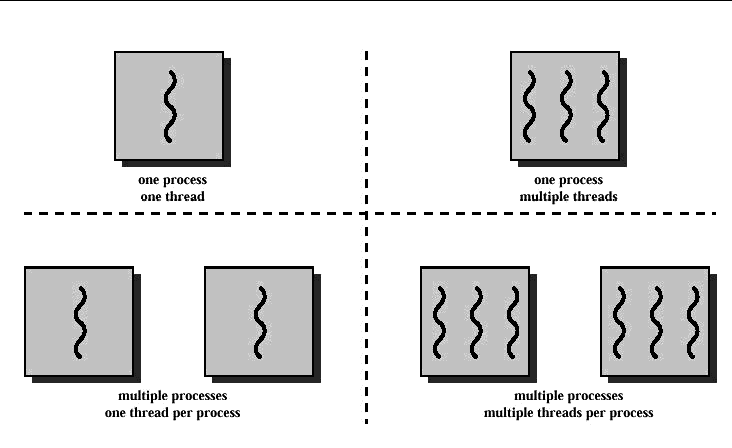
\includegraphics[width=\textwidth]{images/mthread.png}
\end{center}
\end{frame}

\begin{frame}
\frametitle{Thread States}
\begin{changemargin}{1cm}
Conceptually, a thread can be in one of three states:
\begin{itemize}
	\item \textbf{Executing}
	\item \textbf{Ready}
	\item \textbf{Blocked}
\end{itemize}
\end{changemargin}
\end{frame}

\begin{frame}
\frametitle{About Multithreading}
\begin{changemargin}{1cm}
Very few programs written today are single threaded.

It is typical to separate UI from processing. \mnote{Why? See next slides}

Example: File Transfer (FTP) program. \mnote{If the user interface and upload method share a thread, once a file upload has started, the user will not be able to use the UI anymore (and Windows will put the dreaded ``(Not Responding)'' at the end of its dialog title)}
\end{changemargin}
\end{frame}


\begin{frame}
\frametitle{Not Responding}
\begin{changemargin}{3cm}
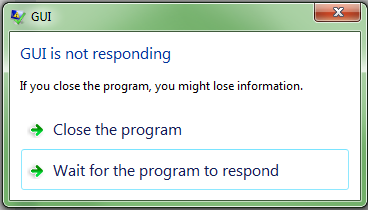
\includegraphics[width=0.5\textwidth]{images/notresponding.png}\\
(From StackOverflow.com)
\end{changemargin}
\end{frame}

\begin{frame}
\frametitle{Not Responding}
\begin{changemargin}{3cm}
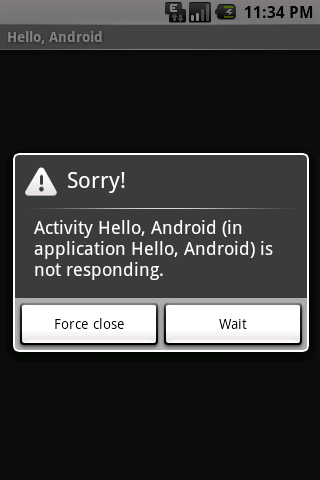
\includegraphics[width=0.45\textwidth]{images/anr.png}\\
(From linuxtopia.org)
\end{changemargin}
\end{frame}

\begin{frame}
\frametitle{Multithreading: FTP}
\begin{changemargin}{1cm}
Solution? Multithreading

When an upload is ready to start, a new thread is created.

Thread runs in the background.

UI Thread does not wait for the upload.

Android official guide says to use this.

\end{changemargin}
\end{frame}

\begin{frame}
\frametitle{Inter-Process Communication}
\begin{changemargin}{1cm}
In most modern OSes, each process runs as if it's in its own world.

If this was not the case, processes could read memory of other processes!

Can still happen in embedded systems.
\end{changemargin}
\end{frame}

\begin{frame}
\frametitle{Inter-Process Communication}
\begin{changemargin}{1cm}
Because of the ``walls'' between processes, communication is hard.

Alternative: communicate between multiple threads!

No enforcement of rules by the OS between threads.
\end{changemargin}
\end{frame}

\begin{frame}
\frametitle{Inter-Process Communication}
\begin{changemargin}{1cm}
Alternative: \alert{Inter-Process Communication} (IPC)

Used for data sharing, message passing, function calls.

Can be set up with files, shared memory, etc.

\end{changemargin}
\end{frame}

\begin{frame}
\frametitle{Android IPC}
\begin{changemargin}{1cm}
\alert{Intents}: used to ask another process to do something.

Explicit: Specify what process should handle the Intent.

Implicit: Ask OS to find programs that can handle the Intent.

If there is more than one, user gets a popup asking to choose.

Example: YouTube link can open in Browser or YouTube App.

\end{changemargin}
\end{frame}

\begin{frame}
\frametitle{Android IPC}
\begin{changemargin}{1cm}
Intent is one way, but there is an alternative.

\alert{Binder}: client-server model for comunication.

Details of the Binder are beyond the scope of this course.

\end{changemargin}
\end{frame}


\begin{frame}
\frametitle{Processes vs. Threads}
\begin{changemargin}{1cm}
Threads ware faster to create and destroy than processes.

Less time to switch between threds in the same process.

Threads within the same process share memory and files.\\
\quad Can communicate easily.

\end{changemargin}
\end{frame}

\begin{frame}
\frametitle{Processes vs. Threads}
\begin{changemargin}{1cm}
No protection between threads in the same process.

If any thread encounters an error, whole process will be halted;
\quad Independent processes can keep going if a related one stops.

\end{changemargin}
\end{frame}


\begin{frame}
\frametitle{Multithreading: Execution}
\begin{changemargin}{1cm}
Assume a computer with 1 processor; 1 thread at a time

Still support multiple threads.

Time division: task switching.

Picture 3 threads. \mnote{ So thread 1 would execute for 20 ms, then thread 2 for 20 ms, then thread 3 for 20 ms, then back to thread 1 for 20 ms.}

User perception: threads executing in parallel \mnote{task switches are so fast the user can't notice them}


\end{changemargin}
\end{frame}


\begin{frame}
\frametitle{Multithreading: Execution}
\begin{changemargin}{1cm}
Now: desktops, laptops, cell phones: multicore processors.

Multicore = multiple threads executing at once.\mnote{The Samsung Galaxy S4 has a quad-core processor and may be executing four different instructions from four different threads at the same time}

Time slicing still occurs if needed. \mnote{if there are 10 threads running on a quad-core system, time slicing is necessary to run all those programs.}

\end{changemargin}
\end{frame}

\begin{frame}
\frametitle{Multithreading}
\begin{changemargin}{1cm}

Two kinds of multithreading: \alert{Co-operative} and \alert{Pre-emptive}

\end{changemargin}
\end{frame}


\begin{frame}
\frametitle{Co-operative Multithreading}
\begin{changemargin}{1cm}

Used to be fairly common - even in Mac OS 9.

Threads yield the CPU.

Problem: greedy threads (never yield). \mnote{It only takes a small number of misbehaving programs to make the system unusable (or just very unpleasant to use) for others.}

\end{changemargin}
\end{frame}

\begin{frame}
\frametitle{Pre-Emptive Multithreading}
\begin{changemargin}{1cm}

Solution: let the OS decide when thread switch.

Every thread acts as if it's the only one.

No need to decide when is a good time to yield.

OS forces a thread switch when it is time.

\end{changemargin}
\end{frame}

\begin{frame}
\frametitle{Pre-Emptive vs Co-operative}
\begin{changemargin}{1cm}

Usually you will see Pre-Emptive.

Embedded systems might not manage threads; might have to use co-operative.

Co-operative an be more efficient if everyone plays nicely.

However, one rogue thread can wreck it for everyone.

\end{changemargin}
\end{frame}

\begin{frame}
\frametitle{Parallelism}
\begin{changemargin}{1cm}

Multiple threads at the same time = tasks completed faster?

\end{changemargin}
\end{frame}

\begin{frame}
\frametitle{Parallelism}
\begin{changemargin}{1cm}

Depends on the nature of the task!

Fully paralellized: 2 $\times$ Threads = 2 $\times$ Speed \mnote{Imagine painting an apartment. It would take one person 12 hours to paint the whole apartment and two people could complete the job in 6 hours.}

Partially paralellized: 2 $\times$ Threads = $(1 < n < 2)$ $\times$ Speed \mnote{Doubling the workers doesn't result in completing the job in half the time. Two chefs working together in a kitchen might take 75\% of the time it would take one chef to cook a meal. Adding the extra worker to the kitchen improved the speed at which food was prepared, but it's not doubled. The chefs can work independently some of the time, but at other times one has to wait for the other; the sauce cannot be put on the chicken until the chicken comes out of the oven.}

Cannot be paralellized: 2 $\times$ Threads = $1$ $\times$ Speed \mnote{no amount of extra workers will speed it up. Some tasks can only be done sequentially. As the folk saying goes, ``Nine women can't have a baby in one month.''}

\end{changemargin}
\end{frame}


\begin{frame}
\frametitle{Multithreading Bugs}
\begin{changemargin}{1cm}

Challenging to convert single threaded code to multithreaded. \mnote{Ideally it should be designed this way from the start}

Multithreaded programs are prone to new types of bugs.\mnote{The most likely problem when working with multiple threads is two or more threads trying to update the same piece of data at the same time.}

Multithreaded bugs will come up later in the course, but we'll take time for a short preview.

\end{changemargin}
\end{frame}

\begin{frame}
\frametitle{Debugging Parallel Programming}
\begin{changemargin}{1cm}

Let's imagine we have an instance of an object \texttt{Location} that has two co-ordinates, \texttt{x} and \texttt{y}. 


\texttt{location.setX(5);\quad\quad location.setX(10);}
\texttt{location.setY(7);\quad\quad location.setY(0);}

\end{changemargin}
\end{frame}

\begin{frame}
\frametitle{Location Example}
\begin{changemargin}{1cm}
Even if each method is atomic, we cannot guarantee an order.

Consider this order:
\begin{enumerate}
	\item Set \texttt{x} to 5
	\item Set \texttt{x} to 10
	\item Set \texttt{y} to 0
	\item Set \texttt{y} to 7
\end{enumerate} 

Result: $(10, 7)$ - Inconsistent! \mnote{Now our data is inconsistent! There was never a location of  in our data set - it should be either $(5, 7)$ or $(10, 0)$, but not half of one and half of another.}

We'll see how to solve this when we get to debugging.

\end{changemargin}
\end{frame}


\begin{frame}
\frametitle{Example: RaceCondition} 
\begin{changemargin}{1cm}

Now we'll examine in Eclipse some code examples where we have a race condition. 

(See the code examples folder in Learn for the source.)


\end{changemargin}
\end{frame}


\end{document}

